\begin{chapter}{Introduction}
    \label{chap:intro}

    \section{Cloud computing models}
    Between the various types of cloud computing architectures, in the last few years have
    emerged three main models, through which to develop web applications. These are IaaS,
    PaaS e SaaS.
    Each of the models is characterized by an increasing level of abstraction regarding
    the underlying infrastructure.

    \begin{figure}
        \centering
        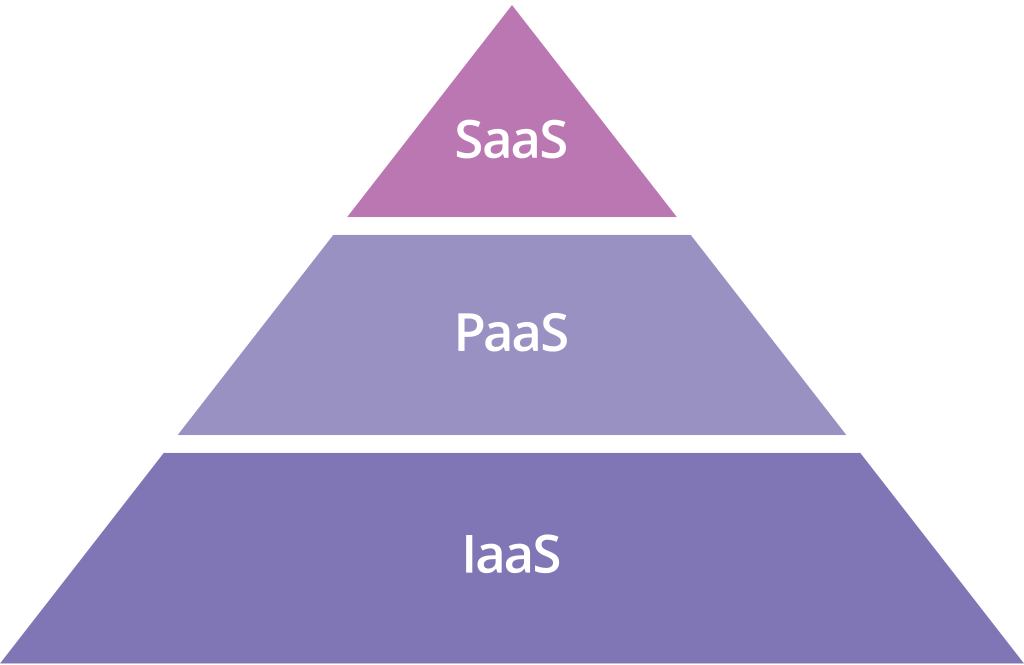
\includegraphics[height=4cm]{source/images/saas-paas-iaas-cloud-pyramid.png}
        \caption{IaaS, PaaS, Saas pyramid}
        \label{fig:cloud_computing_pyramid}
    \end{figure}

    \paragraph{Infrastructure as a Service (IaaS)}
    Infrastructure refers to the computers and servers than run code and store data. A
    vendor hosts the infrastructure in data centers, referred to as the cloud, while
    customers access it over the Internet. This eliminates the need for customers to own
    and manage the physical infrastructure, so they can build and host web applications,
    store data or perform any kind of computing with a lot more flexibility.
    An advantage of this approach is scalability, as customers can add new servers on demand,
    every time the business needs to scale up, and the same apply also if the resources are
    not needed anymore. Essentially servers purchasing, installing, maintenance and updating
    operations are outsourced to the cloud provider, so customers can spend fewer resources
    on that and focus more on business operations, thus leading to a faster time to market.
    The main drawback of this approach is the cost effectiveness, as businesses needs to
    over-purchase resources to handle usage spikes, this leads to wasted resources.

    \paragraph{Platform as a Service (PaaS)}
    This model simplify web development, from a developer perspective, as they can rely on
    the cloud provider for a series of services, which are vendor dependent. However some
    of them can be defined as core PaaS services, and those are: development tools,
    middleware, operating systems, database management, and infrastructure.
    PaaS can be accessed over any internet connection, so developers can work on the
    application from anywhere in the world and build it completely on the browser. This kind
    of simplification comes at the cost of less control over the development environment.

    \paragraph{Software as a Service (SaaS)}
    In this model the abstraction from the underlying infrastructure is maximized. The vendor
    makes available a fully built cloud application to customers, through a subscription
    contract, so rather than purchasing the resource once there is a periodic fee.
    The main advantages of this model are: access from anywhere, no need for updates or
    installations, scalability, as it's managed by the SaaS provider, cost savings.
    However there are also main disadvantages, that makes this solution not suitable in
    some cases: developers have no control over the vendor software, the business may become
    dependent on the SaaS provider (vendor lock-in), no direct control over security, this
    may be an issue especially for large companies.

    \begin{figure}
        \centering
        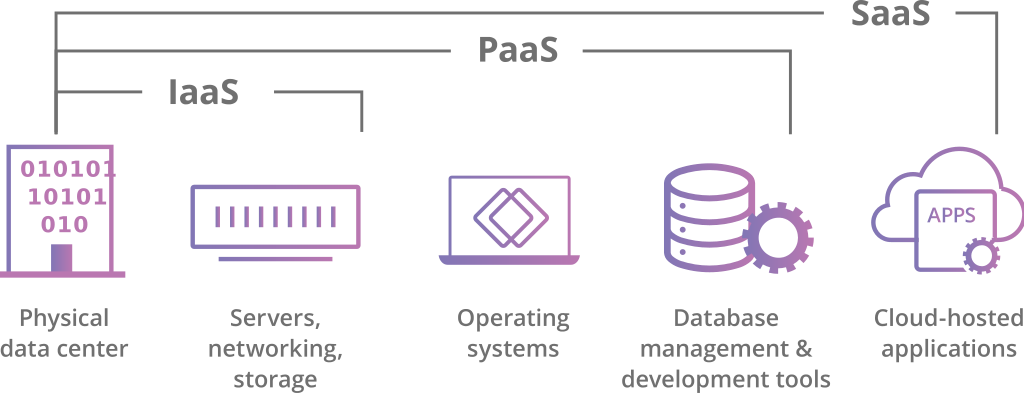
\includegraphics[width=\linewidth]{source/images/saas-paas-iaas-diagram.png}
        \caption{IaaS, PaaS, Saas diagram}
        \label{fig:cloud_computing_architectures}
    \end{figure}

    Another model has recently been added to the three main cloud computing models, named
    Backend as a Service (Baas). This model stands, with some differences, at the same
    level of PaaS, and it's suited especially for web and mobile backend development.
    As with PaaS, BaaS also makes the underlying server infrastructure transparent
    from the developer point of view, and also provides the latter with api and sdk
    that allow the integration of the required backend functionalities.
    The main functionalities already implemented by BaaS are: database management,
    cloud storage, user authentication, push notifications, remote updating and hosting.
    Thanks to these functionalities there may be a greater focus on frontend or mobile
    development.
    In conclusion BaaS provides more functionalities with respect to the PaaS model,
    while the latter provides more flexibility.

    \section{Serverless paradigm}
    The downsides of the previously described approaches varies from the control on the
    infrastructure and on the software, to scalability problems, to end with cost
    and resources utilization effectiveness.
    With the aim of solving these problems, the major providers started investing on
    a new cloud computing model, named Function as a Service (FaaS) and based on the
    serverless paradigm.
    Such a paradigm is based on providing backend services on an as-used basis, with
    the cloud provider allowing to develop and deploy small piece of code without
    the developer having to deal with the underlying infrastructure.
    So despite the terminology, serverless does not means without servers, as they are
    of course still required, but they are transparent to developers, which can focus
    on smaller pieces of code.
    With this model, rather than over purchase the resources, to ensure correct
    functionality in all workload situations, as happens in the IaaS model, the vendor
    charges for the actual usage, as the service is auto-scaling. Thanks to this approach
    consumer costs will be fine grained as shown in \ref{fig:serverless_benefits}.

    \begin{figure}
        \centering
        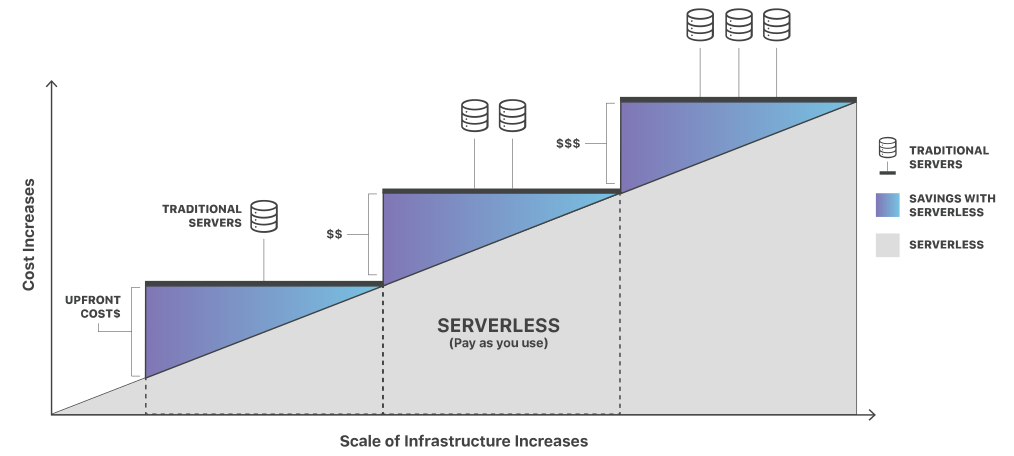
\includegraphics[width=\linewidth]{source/images/benefits-of-serverless.png}
        \caption{Cost Benefits of Serverless}
        \label{fig:serverless_benefits}
    \end{figure}

    Being the underlying infrastructure transparent for the developer, you get the advantage
    of a simpler software development process, and this advantage characterize also
    the PaaS model. Furthermore being the service auto-scaling, is possible to obtain
    a virtually unlimited scaling capacity, as it happens in the IaaS model, where the
    limit is the cloud provider availability.

    An implementation of the serverless paradigm is the cloud model named Function
    as a Service (Faas), which allows developers to write and update pieces of code
    on the fly, typically a single function.
    Such code is then executed in response to an event, usually an api call, but other
    options are possible, so it executed regardless of the events, and this lead to
    the previously described benefit regarding scalability and cost effectiveness.
    Furthermore, through this model turns out to be more efficient to implement web
    applications using the modular approach of the micro services architecture
    (\ref{fig:monolithic_to_microservices}), since the code is organized as a set of
    independent functions from the beginning.

    \begin{figure}
        \centering
        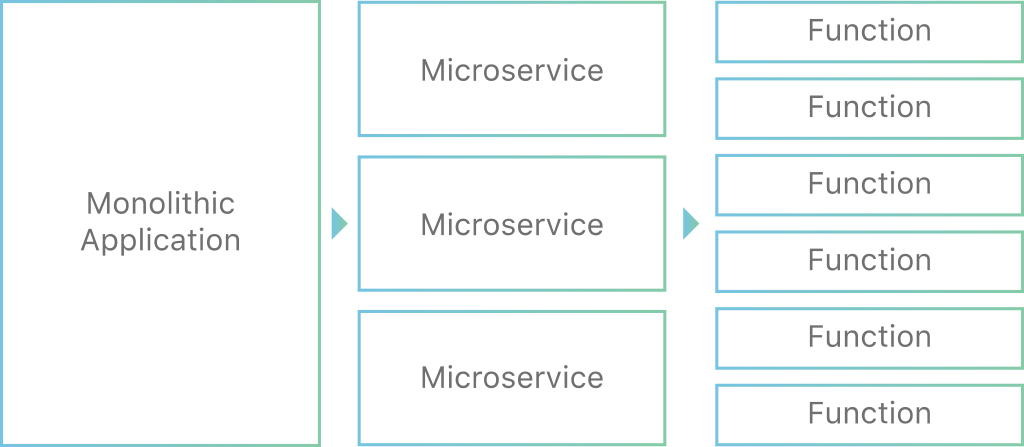
\includegraphics[width=\linewidth]{source/images/monolithic-application-microservice-faas.png}
        \caption{Monolithic to Micro services application}
        \label{fig:monolithic_to_microservices}
    \end{figure}

    So the main advantages of the FaaS model are: improved developer velocity,
    built-in scalability and cost efficiency. As each approach, there are also drawbacks, in
    this case developers have less control on the system, and an increased complexity when it
    comes to test the application in a local environment.

    The first cloud provider to move into the FaaS director has been Amazon, with the
    introduction of aws lambda in 2014, followed by microsoft and google, with
    azure function and cloud function respectively in 2016.

    \section{Serverless Framework}
    Shortly after the release of the service Aws lambda functions, has been introduced,
    in 2015, the Serverless framework, with the main objective of making development,
    deploy and troubleshoot serverless applications with the least possible overhead.
    The framework consists of an open source Command Line Interface and a hosted
    dashboard, that combined provide developers with serverless application lifecycle
    management.

    Although the serverless framework, given the number of cloud providers supported,
    aim to be platform agnostic, this document will consider primarily the Aws provider,
    for both the usage of the serverless framework and the subsequent development of
    the Restlessness framework. This choice is due to the maturity of the platform with
    respect to what the competitors.
    Serverless supports all runtime provided by Aws, corresponding to the most popular
    programming languages such as: Node.js, Python, Ruby, Java, Go, .Net, and others
    are on development.
    This document will focus on the Node.js runtime along with the typescript
    programming language.

    The main work units of the framework, according to the FaaS model, are the functions.
    Each function is responsible for a single job, and although is possible to perform
    multiple tasks using a single function, it's not recommended as stated by the design
    principle Separation of concerns.
    Each function is executed only when triggered by and Event, there are a lot of events,
    such as: http api request, scheduled execution and image or file upload.
    Once the developer has defined the function and the events associated to it,
    the framework take care of creating the necessary resources on the provider platform.

    The framework introduces the concept of Services as unit of organization. Each service
    has one or more functions associated to it and a web application can then be composed
    by multiple services. This structure reflects the modular approach of the micro services
    architecture described previously.
    % @TODO ci potrebbe stare uno schemino per rappresentare meglio servizi e app

    A service is described by a file, located at the root directory of the project, and
    composed in the format \href{https://yaml.org/}{Yaml} or Json.
    Below is a simple serverless.yml file % todo (\ref{fig:...})
    , it defines the service users, which
    contains just a function, responsible of creating a user. The handler field specify
    the path to the function code, in this case the framework will search for a handler.js file,
    exporting a usersCreate function, as show on % todo \ref{fig:...}.

    % @TODO insert also provider etc
    % insert code of a sample serverless.yml file
    % service: users
    % functions:
    %     usersCreate:
    %         handler: handler.usersCreate
    %         events:
    %             - http: post users/create

    % insert code of a sample handler
    % async function usersCreate(event, context) {
    %     const user = { name: 'sample_name', surname: 'sample_surname' }
    %     await mockDb.createUser(user)
    %     return user
    % }

    Serverless is flexible and does not force a fixed structure of the project, that
    task is up to the developer.
    Defined that structure, the service can be deployed using the Serverless CLI, as
    show in % \ref{fig:...}
    % command: $ serverless deploy
    % show also deploy output
    The deploy command creates the necessary aws resources, in this case they are:
    a lambda function corresponding to the usersCreate function and an api gateway to
    handle http requests.
    It is then possible to test the newly created resource by making requests to the
    url returned by the CLI, as shown in % \ref{fig:...} figure of deploy log
    specifying the resource path /users/create.
    It is possible to invoke online functions also directly from the CLI,
    specifying the identifier of the function used in the serverless.yml file, as shown in % \ref{} or code
    % command: $ serverless invoke -f usersCreate
    The development and deploy process shown for a service with a single function
    remains the same as the service complexity grows, in particular it is possible to
    modify and deploy a single function at a time, since each function has its own
    resource associated.
    This process gets along with the previously described micro services architecture.

    \subsection{Advantages}
    The main advantages of using the Serverless framework are:
    \begin{itemize}
        \item Provider agnostic: the framework aims to be independent from the chosen
            cloud provider, thus avoiding vendor lock-in. In practice this feature is
            not achieved completely, as the configuration file serverless.yml may be
            different across providers. However the main structure remains the same,
            and that simplify providers migration.
        \item Simplified development: the CLI commands simplify the development process,
            from the deploy from the testing of the deployed functions.
        \item Extensible: is possible to develop plugins that integrate with the
            CLI commands lifecycle, increasing their functionalities.
        \item Dashboard: the hosted dashboard allow monitoring and tracing of the
            deployed functions and services.
    \end{itemize}

    \subsection{Disadvantages}
    The main advantages of using the Serverless framework and the Serverless paradigm are:
    \begin{itemize}
        \item Compilation of the configuration file may become tedious as the project grows.
        \item The framework is extremely flexible regarding the project structure and
            that is an advantage, however this can also be a drawback as it's up to the
            developer to find a suitable structure, and this means less time spent on
            business related tasks.
        \item Unit testing: it is possible to test a deployed function easily, however
            for big projects, where it's necessary to test a lot of functions, this may
            become cumbersome.
        \item Resource threshold: for projects created with Aws, a single
            serverless.yml file may create up to 200 resources, and if exceeded
            the deploy operation fails. Since each function is responsible for the
            creation of about 10 resources, is very easy to exceed this limit.
            The only solution so solve this problem is to split the functions across
            multiple services, hence different serverless.yml configuration files.
        \item Cold start: inherent overhead of the current implementation of the
            serverless paradigm. Since each function is executed only in response to
            an event, a certain amount of time is required for resources initialization.
    \end{itemize}

    \section{The idea behind Restlessness}
    The Restlessness framework was born with the goal of improving the developer
    experience of the Serverless framework, by addressing its encountered problems.
    The framework is composed by a Command Line Interface and a frontend application
    with an associated web server running locally.
    In particular the main functionalities that the framework aims to provide are:
    \begin{itemize}
        \item Creation of a new project, through the CLI, based on the typescript
            language and with a standard structure.
        \item A local Web Interface that allow creating and managing project resources,
            % todo al posto delle parentesi usare i riferimenti
            functions, with their associated events, and models.
        \item The creation of a standard unit testing structure for each function,
            and based on the \href{https://www.npmjs.com/package/jest}{jest} library.
        \item A standard validation structure for function's input, based on the
            \href{https://www.npmjs.com/package/yup}{yup} library.
        \item Deploy of multiple services with a single CLI command, to deal with
            the resource threshold limitation of Aws.
    \end{itemize}

    By addressing those points the framework aims to give developers the tools to
    focus on writing business code rather than spend time on boundary problems,
    that are important, but there may be the risk of solving the same problems
    multiple times (reinventing the wheel), which may be avoided.

    \section{Related Works}
    @TODO\\
    Are there other similar framework? What are the differences? Why use restlessness instead?

    \section{Tools}
    Several tools were used during the development of the project, varying from the ones supporting
    code development, to the organizational ones. Below is a list of them:

    \paragraph{\href{https://www.github.com}{GitHub}}
    Version control platform based on the Git system. It has been used for the development, organization and
    management of the main project \textit{Restlessness}, as well as the drafting of this document.
    Both are available for consultation:
    \begin{itemize}
        \item Restlessness: \url{https://www.github.com/getapper/restlessness}
        \item Thesis: \url{https://www.github.com/androsanta/Thesis}
    \end{itemize}

    \paragraph{\href{https://slack.com}{Slack}}
    Business communication platform. It has been used for team communication to achieve a more direct
    and private interaction with respect to what \textit{GitHub} offers.

    \paragraph{\href{https://circleci.com}{CircleCi}}
    Continuous integration platform. It has been used for testing and deploying operations
    for all restlessness packages.

    \paragraph{\href{https://www.serverless.com}{Serverless}}
    Open source framework that simplify the development and deployment of applications based on the
    serverless architecture, on the best known compute services.

    \paragraph{\href{https://aws.amazon.com}{Aws}}
    Amazon Web Services. Platform for cloud computing services. It has been used for deployment and
    testing of application created with the \textit{Restlessness} framework.

    \paragraph{\href{https://nodejs.org/en/}{Node.js}}
    Open source Javascript runtime environment that allow Javascript code execution outside a
    web browser.

    \paragraph{\href{https://www.npmjs.com/}{Npm}}
    The \textit{Node.js} package manager. It has been used for project's dependencies
    and for publishing of all \textit{Restlessness} packages.


    \paragraph{\href{https://www.typescriptlang.org/}{Typescript}}
    It extends the Javascript language by adding type definitions, and a transpiler that generates
    code that runs anywhere Javascript runs, from the browser to \textit{Node.js}. It has been the
    main programming language used.

    \paragraph{\href{https://www.jetbrains.com/webstorm}{WebStorm}}
    Javascript IDE from \href{https://www.jetbrains.com}{JetBrains}. It has been used for
    all code development.

\end{chapter}
